\documentclass[12pt,a4paper]{article}
\usepackage[UTF8]{ctex}
\usepackage{graphicx}
\usepackage{geometry}
\usepackage{ulem}
\usepackage{enumitem}
\usepackage{titlesec}
\usepackage{multicol}
\usepackage[export]{adjustbox}
\usepackage{amsmath}  % 推荐用于更好的数学排版
\usepackage[utf8]{inputenc}
\usepackage{CJKutf8}
\usepackage{fancyhdr}
\usepackage{lastpage}
\usepackage{ulem}
\usepackage{tabularx}
\usepackage{float}

% 页眉页脚设置
\pagestyle{fancy}
\fancyhf{} % 清除所有页眉页脚
% 设置页眉内容
%-==========1. 填写从第二页开始 每页第一行的信息==========-
\fancyhead[C]{
    \makebox[4.5em][c]{实验名称：} \uline{\makebox[14em][c]{一阶RC电路瞬态响应过程实验}} 
    \makebox[2.5em][c]{姓名：} \uline{\makebox[4em][c]{}} 
    \makebox[2.5em][c]{学号：} \uline{\makebox[5em][c]{}}
}%--------------------------------------------------------
\fancyfoot[C]{第 \thepage\ 页，共 \pageref{LastPage} 页}

% 取消页眉和页脚的下划线
\renewcommand{\headrulewidth}{0pt} % 页眉横线粗细设为0
\renewcommand{\footrulewidth}{0pt} % 页脚横线粗细设为0

% 调整页眉高度
\setlength{\headheight}{50pt}

% 设置plain样式（用于第一页）
\fancypagestyle{plain}{
    \fancyhf{} % 清除所有页眉页脚
    \renewcommand{\headrulewidth}{0pt} % 隐藏页眉横线
    \fancyfoot[C]{第 \thepage\ 页，共 \pageref{LastPage} 页} % 保留页脚
}
% 设置页面边距
\geometry{left=2.54cm,right=1.5cm,top=2.54cm,bottom=2.54cm}

% 设置正文字体大小为小四
\renewcommand{\normalsize}{\fontsize{12pt}{16pt}\selectfont}
% 设置章节格式
\titleformat{\section}{\fontsize{16pt}{22pt}\selectfont\bfseries}{\thesection}{1em}{} % 一级标题：三号
\titleformat{\subsection}{\fontsize{15pt}{20pt}\selectfont\bfseries}{\thesubsection}{1em}{} % 二级标题：小三

\begin{document}
\thispagestyle{plain}%第一页使用 plain 样式，而不是默认的 fancy 样式，第一页不再显示页眉
% 标题部分 - 两栏布局
\begin{multicols}{2}
    % 左栏：图片和实验报告标题
    % 左栏：使用空行创建前三行
    \noindent
    ~\\ % 第一行
    ~\\ % 第二行
    ~\\ % 第三行
    \hphantom{占位}% 使用空占位符
    \raisebox{-0.5\baselineskip}% 图片向下移动半行
    {
\includegraphics[width=1.85in,height=0.58in]{ZJU.jpg}}
    \hspace{.5em}% 图片和标题之间的间距
    \raisebox{0pt}[\height][0pt]% 标题底部对齐
    {\textbf{\fontsize{26pt}{30pt}\selectfont 实验报告}}
    
    \columnbreak % 换到右栏
    
    % 右栏：个人信息
    % 右栏：个人信息 - 靠右对齐 
%-==========2. 填写个人信息==========-
    \begin{flushright}
        \makebox[3em][l]{专业：} \uline{\makebox[9em][c]{法语-电子科学与技术}} \\
        \makebox[3em][l]{姓名：} \uline{\makebox[9em][c]{}} \\
        \makebox[3em][l]{学号：} \uline{\makebox[9em][c]{}} \\
        \makebox[3em][l]{日期：} \uline{\makebox[9em][c]{2025年11月18日}} \\
        \makebox[3em][l]{地点：} \uline{\makebox[9em][c]{紫金港东四216}} \\
    \end{flushright}   
\end{multicols}
% 课程名称等信息（单栏）
%-==========3. 填写课程信息==========-
\noindent
课程名称： \uline{电子电路设计实验I} \hfill 指导老师： \uline{施红军、叶险峰、邓靖靖} \hfill 成绩： \uline{\hspace{3cm}} \\
实验名称： \uline{一阶RC电路瞬态响应过程实验} \hfill 实验类型： \uline{验证实验} \hfill 同组学生姓名： \uline{}
%-==========4. 正文开始==========-
\section*{一、实验目的}

1、研究一阶RC电路零输入响应和零状态响应的基本规律和特点；

2、学习使用示波器观察、分析一阶RC电路的响应；

3、从响应曲线中求一阶RC电路的时间常数$\tau$；


\section*{二、实验任务与要求}

1、理论计算4个一阶RC电路的时间常数$\tau=RC$。

2、使用示波器观察两种周期、两种占空比共四种不同的方波。

3、更换电路中电阻、电容的大小，用示波器分别观察4个一阶RC电路的零输入响应、零状态响应：

（1）描绘响应曲线（拍照）；

（2）用示波器测量4个RC电路的时间常数$\tau$；

4、比较时间常数的理论值和测试值是否一致。


\section*{三、实验原理}

图\ref{fig1}是一阶RC电路。

\begin{figure}[H]
    \centering
    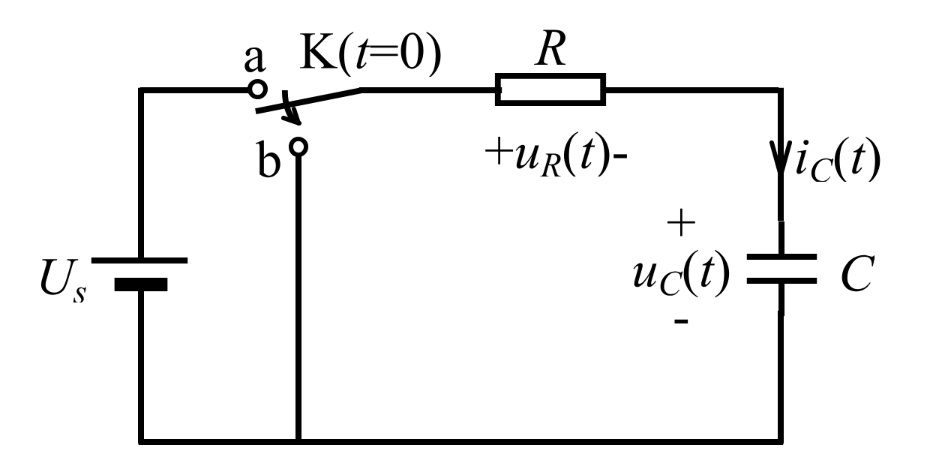
\includegraphics[width=0.4\textwidth, height=0.14\textheight]{RC-1.png}
    \caption{一阶RC电路}
    \label{fig1}
\end{figure}

\textbf{零输入响应}指的是电路在无激励情况下，由储能元件的初始状态引起的响应。

在图\ref{fig1}中，先让开关K合于位置 a，使电容C的初始电压值 \(u_C(0) = U_0\)，再将开关K转到位置b。电容器开始放电，放电方程为：
%%
\[ u_C + RC \frac{du_C}{dt} = 0 \quad (t \geq 0) \]
%%
可以得出电容器上的电压和电流随时间变化的规律：
%%
\[ u_C(t) = u_C(0_e)e^{-\frac{t}{RC}} = U_0 e^{-\frac{t}{\tau}} \quad (t \geq 0) \]
%%
\[ i_C(t) = -\frac{u_C(0_e)e^{-\frac{t}{RC}}}{R} = -\frac{U_0}{R} e^{-\frac{t}{\tau}} \quad (t \geq 0) \]
%%
式中 \(\tau = RC\)，即为时间常数，其物理意义是 \(u_C(t)\) 衰减到 \(1/e\) (36.8\%) \(u_C(0)\) 所需要的时间，反映了电路过渡过程的快慢程度。$\tau$ 越大，暂态响应所持续的时间越长，即过渡过程的时间越长；反之，$\tau$ 越小，过渡过程的时间越短。时间常数 $\tau$ 可通过相应的衰减曲线来获得(见图\ref{fig2}左)。

\begin{figure}[H]
    \centering
    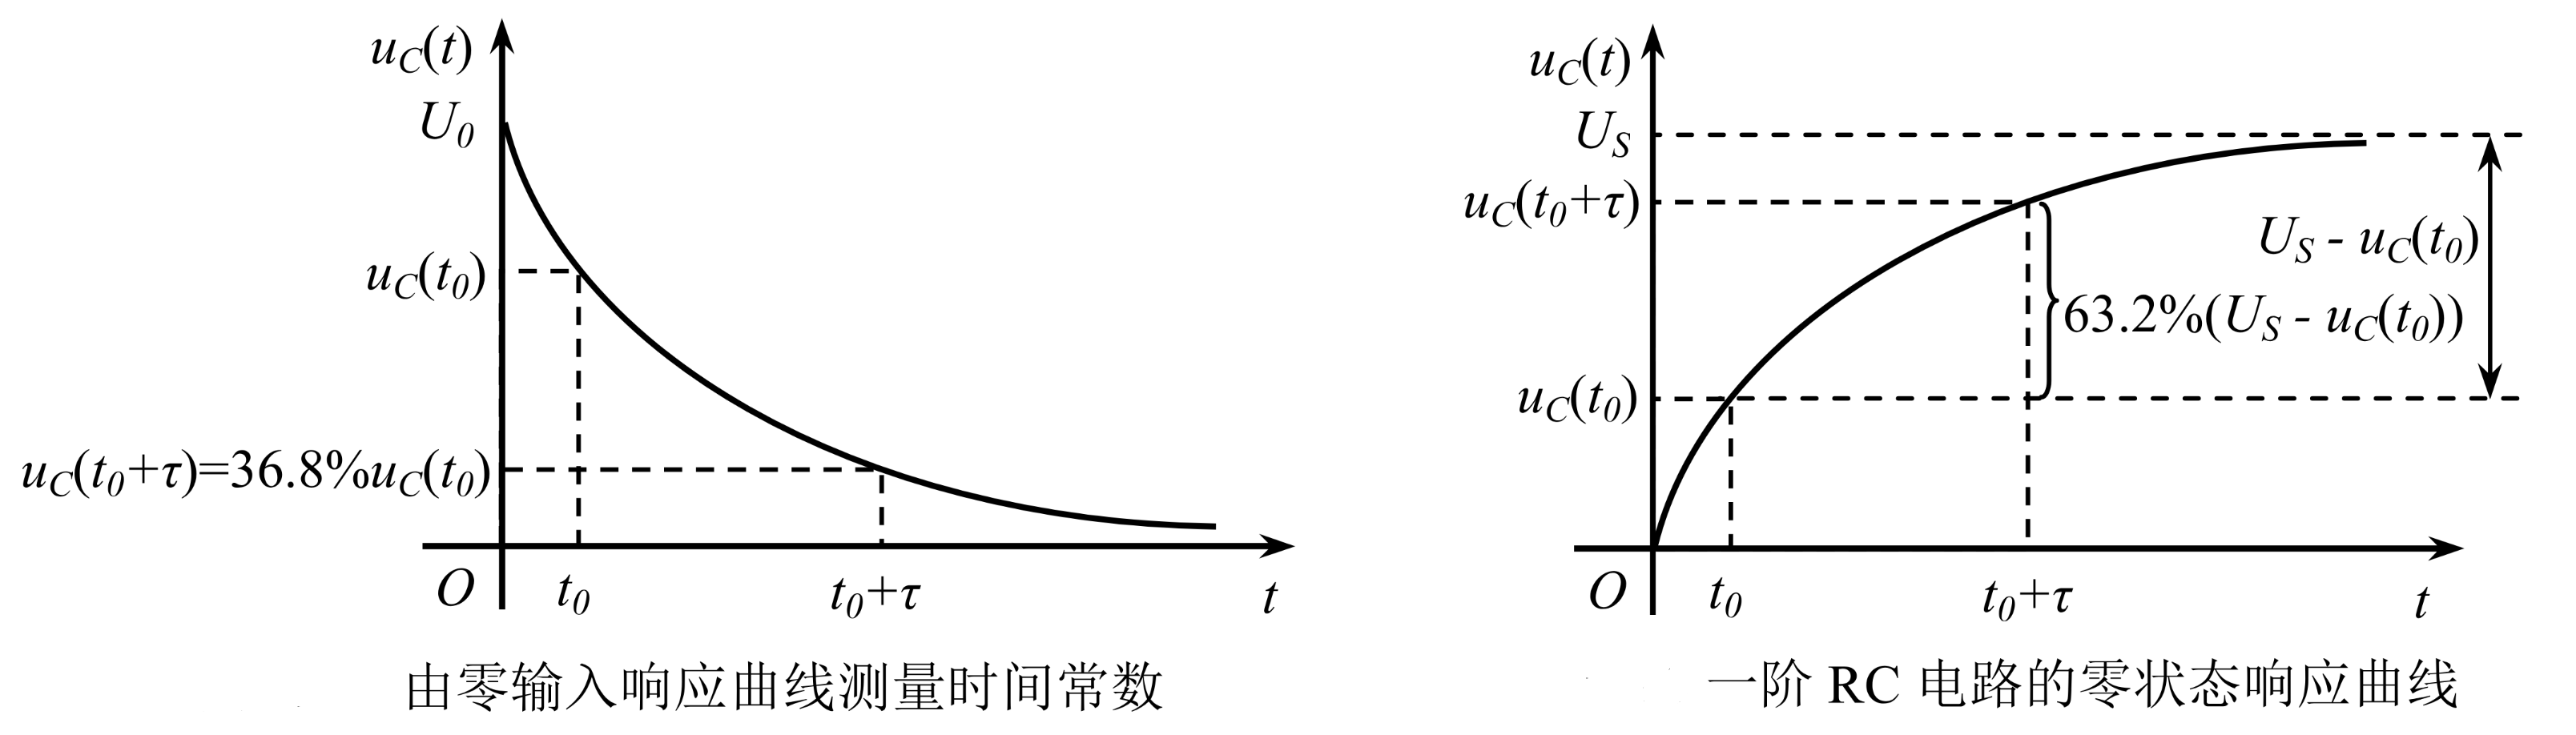
\includegraphics[width=0.94\textwidth, height=0.2\textheight]{RC-2.png}
    \caption{一阶RC电路的零输入/零状态响应曲线}
    \label{fig2}
\end{figure}


数学上的证明：$t_0$时刻下的电容电压
$$u_{c}(t_0)=U_{0}e^{-\frac{t_0}{\tau}}$$
则$t_0+\tau$时刻下
$$u_{c}(t_0+\tau)=U_{0}e^{-\frac{t_0+\tau}{\tau}}=U_{0}e^{-\frac{t_0}{\tau}}e^{-\frac{\tau}{\tau}}=U_{0}e^{-\frac{t_0}{\tau}}\cdot\frac{1}{e}=\frac{1}{e}u_{c}(t_0)$$


\textbf{零状态响应}指的是初始状态为零，而输入不为零所产生的电路响应。

在图\ref{fig1}中，先让开关K合于位置b，当 \( t = 0 \) 时，将开关 K 转到位置a。电容器开始充电，充电方程为：
%%
\[u_c + RC \frac{du_c}{dt} = U_s \quad (t \geq 0)\]
%%
初始值：\( u_c(0) = 0 \)
%%
可以得出电压和电流随时间变化的规律：
%%
\[u_c(t) = U_s \left( 1 - e^{-\frac{t}{RC}} \right) = U_s \left( 1 - e^{-\frac{t}{\tau}} \right) \quad (t \geq 0)\]
%%
\[i_c(t) = \frac{U_s}{R} e^{-\frac{t}{RC}} = \frac{U_s}{R} e^{-\frac{t}{\tau}} \quad (t \geq 0)\]
%%
\(\tau = RC\) 为时间常数，其物理意义是由初始值上升至稳态值与初始值差值的63.2\%处所需的时间。同样可以从响应曲线中求得时间常数\(\tau\)(见图\ref{fig2}右)。

\section*{四、实验方案设计与参数计算}

\subsection*{4.1 实验电路}






\begin{figure}[H]
    \centering
    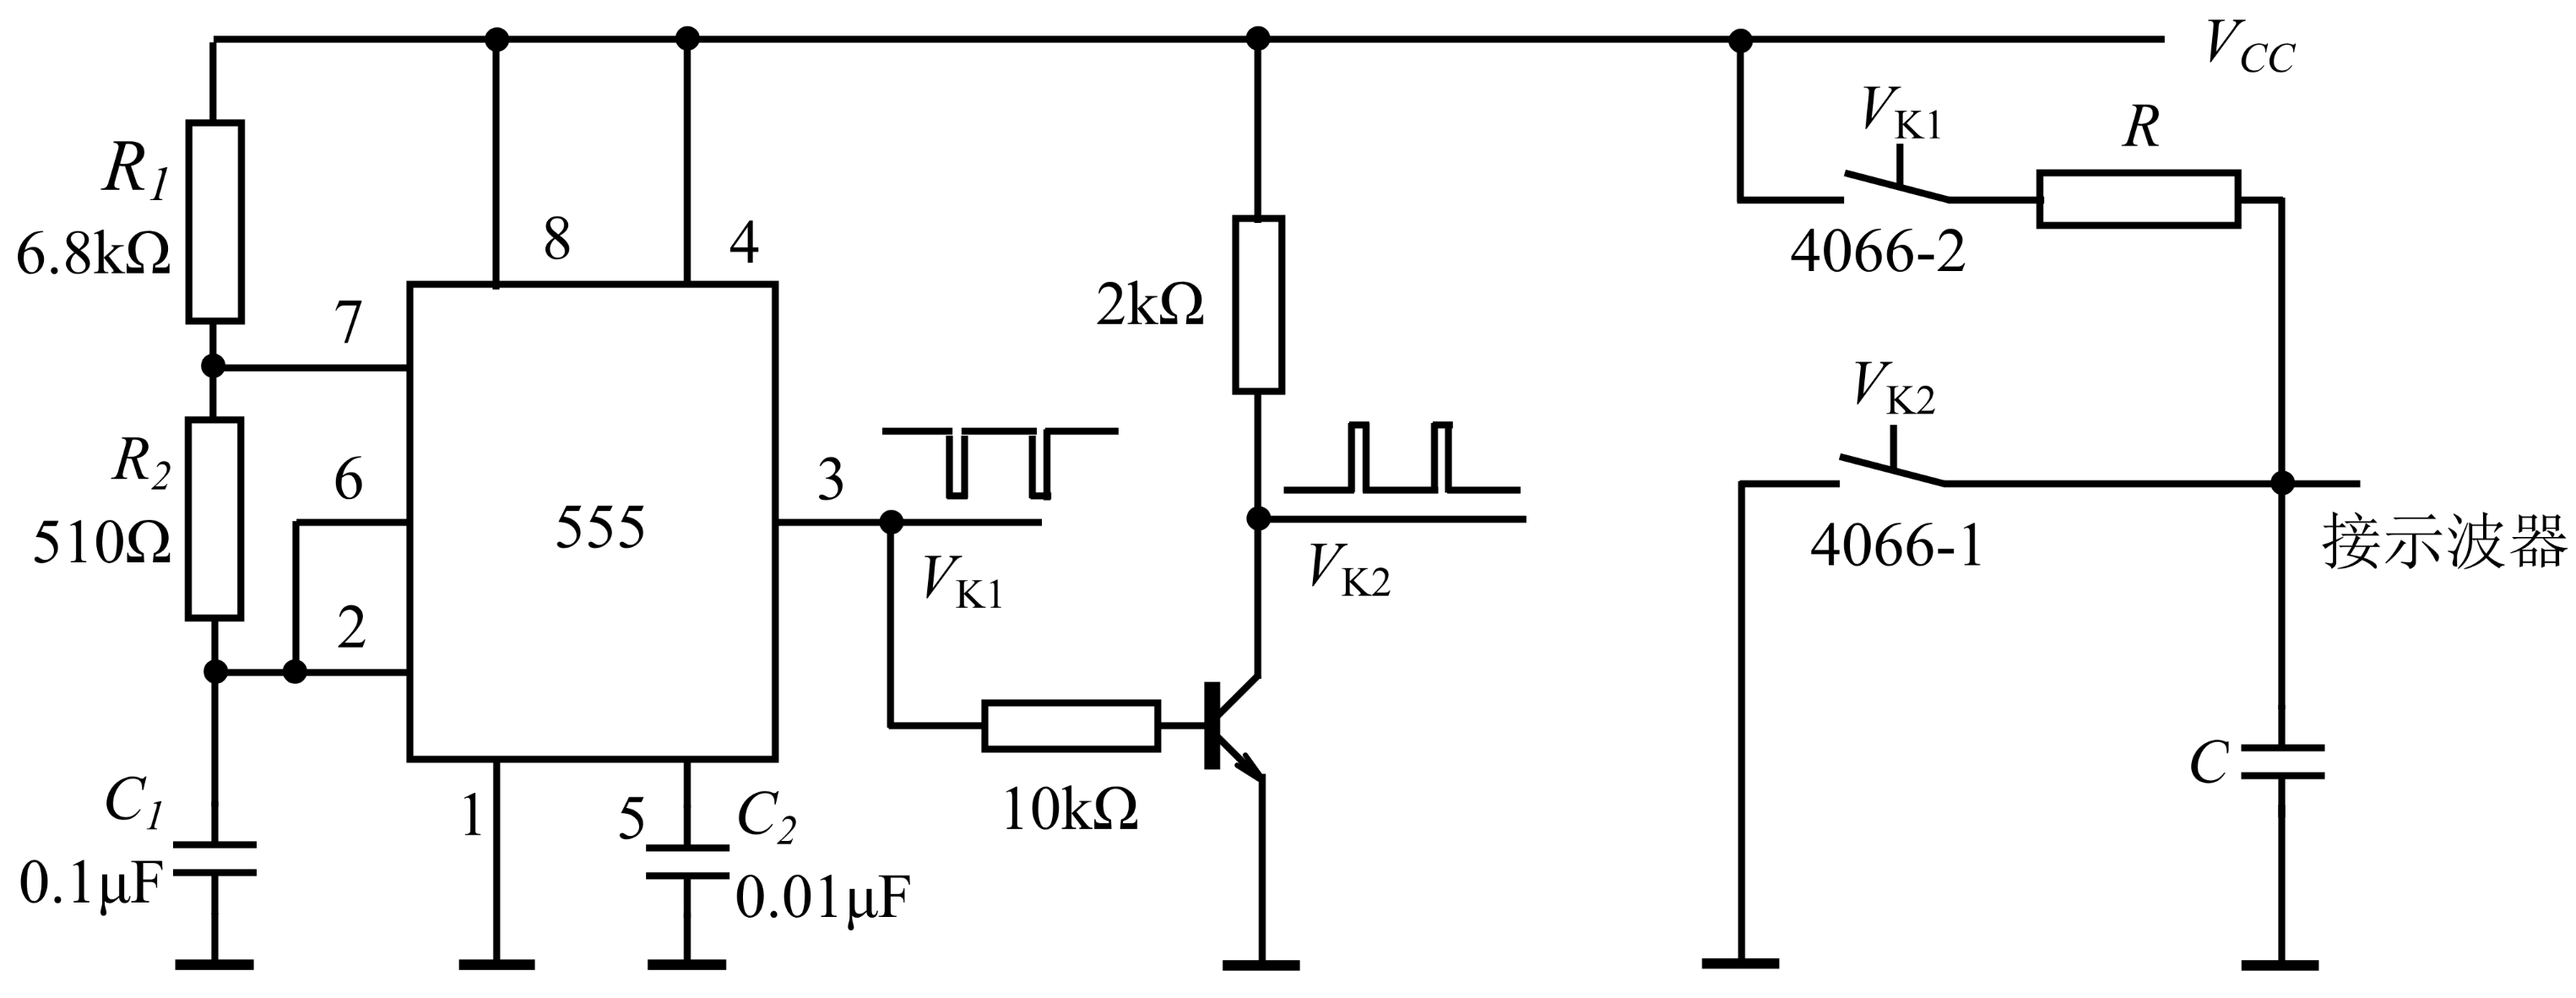
\includegraphics[width=0.75\textwidth, height=0.2\textheight]{circuit-2.png}
    \caption{重复激励的零状态响应观测的实验电路}
    \label{fig3}
\end{figure}

RC电路的响应是一个十分短暂的单次变化瞬态过程，一次激励引起电路一次响应。要在示波器上显示RC电路的响应曲线进而进行观察和测量有关参数，就必须周期性地重复进行激励，使这种单次变化的过程重复出现，而且要保证激励信号与示波器扫描的同步，只有这样，才能在示波器上显示稳定的电路响应曲线。

为此，实验时必须设计一个实验方案，实现对RC电路的周期性重复激励和向示波器提供扫描同步信号。图\ref{fig3}是观测零状态响应过程的实验电路，选用555时基电路作激励脉冲信号发生电路，用CD4066电子开关实现电路中开关的切换，脉冲信号的前沿为示波器提供扫描同步触发信号。

\subsection*{4.2 理论计算}

计算4个一阶RC电路的时间常数$\tau=RC$，算出$5\tau$,并据此选择合适的方波周期，当方波半周期$T/2<5\tau$时，将不能观察到完整的响应过程。

\begin{table}[H]
\centering
\caption{时间常数理论计算值} 
\renewcommand{\arraystretch}{1.2}
\small
\begin{tabular}{|p{1.2cm}|p{1.2cm}|p{1.2cm}|p{1.2cm}|p{2.8cm}|}
\hline
 $R/\mathrm{k}\Omega$ & $C/\mathrm{nF}$ & $\tau$/ms & $5\tau$/ms &激励源周期选择\\
\hline
9.1 & 100 &   0.910& 4.55& 5ms\\
\hline
0.75 & 100 &   0.075& 0.375&0.5ms\\
\hline
4.3 & 220 &   0.946 & 4.73&5ms\\
\hline
4.3 & 10 &   0.043& 0.215&0.5ms\\
\hline
\end{tabular}

\end{table}


\begin{figure}[H]
    \centering
    
\includegraphics[width=0.8\textwidth, height=0.34\textheight]{5.jpg}
    \caption{方波周期选择不合适}
    \label{fig15}
\end{figure}

\section*{五、实验仪器设备}

直流稳压电源、示波器。

\section*{六、实验步骤、调试过程、实验数据记录}

更换电路中电阻、电容的大小，用示波器分别观察4个一阶RC电路的零输入响应、零状态响应：

1、描绘响应曲线（拍照）。

下面列出了四个RC电路的响应曲线。

\begin{figure}[H]
    \centering
    
\includegraphics[width=0.8\textwidth, height=0.34\textheight]{2.jpg}
    \caption{$R=9.1\mathrm{k}\Omega,C=100\mathrm{nF}$时的零状态响应曲线}
    \label{fig11}
\end{figure}

\begin{figure}[H]
    \centering
    
\includegraphics[width=0.8\textwidth, height=0.34\textheight]{1.jpg}
    \caption{$R=0.75\mathrm{k}\Omega,C=100\mathrm{nF}$时的零状态响应曲线}
    \label{fig12}
\end{figure}

\begin{figure}[H]
    \centering
    
\includegraphics[width=0.8\textwidth, height=0.34\textheight]{4.jpg}
    \caption{$R=4.3\mathrm{k}\Omega,C=220\mathrm{nF}$时的零输入响应曲线}
    \label{fig13}
\end{figure}

\begin{figure}[H]
    \centering
    
\includegraphics[width=0.8\textwidth, height=0.34\textheight]{3.jpg}
    \caption{$R=4.3\mathrm{k}\Omega,C=10\mathrm{nF}$时的零输入响应曲线}
    \label{fig14}
\end{figure}


2、用示波器测量4个RC电路的时间常数。

对于\textbf{零状态响应}，测量方法如下：

（1）在零状态响应曲线上，任意选取一点 \((t_0, u_c(t_0))\)；

（2）则经过时间 \(\tau\) 后，电容电压为  
\[u_c(t_0 + \tau) = 63.2\% \left( U_S - u_c(t_0) \right) + u_c(t_0)\]

（3）寻找曲线上数值为 \(u_c(t_0 + \tau)\) 的点；

（4）该点在 \(t\) 轴上的投影，与 \(t_0\) 之间的差值即为 \(\tau\)。

\begin{table}[H]
\centering
\caption{零状态响应时间常数测量计算过程（单位：电压/V，时间/$\mu$s）} 
\renewcommand{\arraystretch}{1.2}
\small
\begin{tabular}{|p{1.2cm}|p{1.2cm}|p{1.2cm}|p{2cm}|p{4.5cm}|p{1.2cm}|p{1.2cm}|}
\hline
$U_S$& $u_{c}(t_0)$ & $t_0$ &$U_S-u_{c}(t_0)$ &$63.2\%(U_S-u_{c}(t_0))+u_{c}(t_0)$& $t_0+\tau$ & $\tau$ \\
\hline
11.26 &4.67 &-140 &6.59 &8.835 &740 &880 \\
\hline
11.34 &3.596 &-26 &7.744 &8.490 &52 &78 \\
\hline

\end{tabular}

\end{table}

对于\textbf{零输入响应}，测量方法如下：

（1）在零输入响应曲线上，任意选取一点 \((t_0, u_c(t_0))\)；

（2）则经过时间 \(\tau\) 后，电容电压为 
\[u_c(t_0 + \tau) = 36.8\%u_c(t_0)\]

（3）寻找曲线上数值为 \(u_c(t_0 + \tau)\) 的点；

（4）该点在 \(t\) 轴上的投影，与 \(t_0\) 之间的差值即为 \(\tau\)。



\begin{table}[H]
\centering
\caption{零输入响应时间常数测量计算过程（单位：电压/V，时间/$\mu$s）} 
\renewcommand{\arraystretch}{1.2}
\small
\begin{tabular}{|p{1.2cm}|p{1.2cm}|p{2cm}|p{1.2cm}|p{1.2cm}|}
\hline
 $u_{c}(t_0)$ & $t_0$ &$36.8\%u_{c}(t_0)$& $t_0+\tau$ & $\tau$ \\
\hline
8.182 &780 &3.011 &1760 &980 \\
\hline
8.105 &60 &2.983 &104 &44 \\
\hline

\end{tabular}

\end{table}

至此得到四个一阶RC电路的时间常数测量值。

\begin{table}[H]
\centering
\caption{时间常数测量值} 
\renewcommand{\arraystretch}{1.2}
\small
\begin{tabular}{|p{1.2cm}|p{1.2cm}|p{2.4cm}|p{2.4cm}|}
\hline
 $R/\mathrm{k}\Omega$ & $C/\mathrm{nF}$ & $\tau$测量值/ms& $\tau$计算值/ms\\
\hline
9.1 & 100 & 0.880 & 0.910 \\
\hline
0.75 & 100 & 0.078 & 0.075\\
\hline
4.3 & 220 & 0.980 & 0.946 \\
\hline
4.3 & 10 & 0.044 & 0.043\\
\hline
\end{tabular}

\end{table}

\section*{七、数据分析与讨论}

四个一阶RC电路的时间常数测量值与理论值之间存在误差，主要来源于：

1、示波器的取值精度（仪器误差）

时间基准精度： 示波器水平轴（时间轴）的采样率和时基设置决定了时间测量的最小分辨率。例如，当时基设置为1ms/div时，肉眼从屏幕上读出的时间值精度可能只有0.1ms左右。

电压测量精度： 在测量时间常数$\tau$时，我们通常寻找电容电压上升至电源电压的63.2\%（充电）或下降至36.8\%（放电）的那个点。示波器垂直轴的电压分辨率以及ADC的精度会影响这个电压点的判断。

系统固有误差： 示波器本身和探头也存在固有的响应时间和精度限制。

2、实验者的视觉误差（人为误差）

光标对齐误差： 这是最主要的视觉误差。当使用示波器的光标功能来测量63.2\%电压点对应的时间时，人眼很难将光标线完美地对准曲线的精确位置和电压的精确高度。

但误差较小，可以认为测量值与理论值基本一致。至此我们用实验证明了一阶RC电路的时间常数$\tau=RC$。


\section*{八、结论}

在一阶RC电路零输入响应、零状态响应中时间常数的物理意义即电阻阻值和电容值的乘积，即$\tau=RC$。


\section*{九、心得与体会}

在本次实验中，我学会了如何用示波器测量电路的时间常数，并用实验数据验证了时间常数的物理意义。我也认识到实验前的准备是十分重要的，只有充分准备才能保证实验的准确性和可靠性。我还认识到，在实验中出现异常时，需要耐下心来逐个模块进行测试，以排除可能的故障。

\section*{十、思考题}

\textbf{1、什么是零输入响应、零状态响应？}

零输入响应：指电路中没有外部激励（即输入为零），仅由电路中动态元件（如电容、电感）的初始储能（如电容电压、电感电流）所引起的响应。

零状态响应：指电路中动态元件的初始状态为零（初始储能为零），仅由外部激励所引起的响应。

\textbf{2、在用示波器观察 RC 电路响应时如何才能使示波器的扫描与电路激励同步？}

为了使示波器的扫描与电路激励同步，应将示波器的触发源 (Trigger Source) 设置为外部触发模式，并使用电路中的激励信号作为触发信号。这样，每次扫描都从激励信号的特定点（如上升沿或下降沿）开始，从而在屏幕上显示稳定的波形。

\textbf{3、什么是时间常数？它在电路中起什么作用？}

时间常数$\tau$是表征一阶电路（如RC或RL电路）瞬态过程进行快慢的物理量。对于RC电路，$\tau=RC$;对于RL电路，$\tau=L/R$。它决定了电路充放电过程的速度。时间常数$\tau$越大，瞬态过程（如电容充电或放电）进行得越慢；反之则越快。理论上，电路需要大约$5\tau$的时间才能达到稳定状态。



\end{document}